
\section*{C}


\subsection*{Typen und Print Ausgabe}

\begin{tabular}{|c|c|c|c|c|c|c|c|c|}
\cline{1-3} \cline{5-6} \cline{8-9} 
char & 1B & $-128$ bis $127$ &  & \textbf{Zahl} & \textbf{Interpretation} &  & \textbf{ph} & \textbf{interpret}\tabularnewline
\cline{1-3} \cline{5-6} \cline{8-9} 
int & 4B & $-2^{31}$ bis $2^{31}$ &  & 037 & oktal Zahl &  & \%d, \%i & int\tabularnewline
\cline{1-3} \cline{5-6} \cline{8-9} 
float & 4B & $-3.4\times10^{38}$ bis $3.4\times10^{38}$ &  & 0x23 & hexdezimal Zahl &  & \%u & unsigend int\tabularnewline
\cline{1-3} \cline{5-6} \cline{8-9} 
double & 8B & $-1.79\times10^{308}$ bis $1.79\times10^{308}$ &  & 3.215f & Float &  & \%c & char\tabularnewline
\cline{1-3} \cline{5-6} \cline{8-9} 
unsigned char & 1B & $0$ bis $255$ &  & 0 / other & false / true &  & \%s & char{*} (String bis \textbackslash{}0)\tabularnewline
\cline{1-3} \cline{5-6} \cline{8-9} 
unsigned int & 4B & $0$ bis $2^{32}-1$ &  & stdin & Tastatur &  & \%f & double, float\tabularnewline
\cline{1-3} \cline{5-6} \cline{8-9} 
short (int) & 2B & $-32768$ bis $32767$ &  & stdout & Konsole &  &  & \tabularnewline
\cline{1-3} \cline{5-6} \cline{8-9} 
unsigned short (int) & 2B & $0$ bis $65535$ &  & stderr & Konsole &  &  & \tabularnewline
\cline{1-3} \cline{5-6} \cline{8-9} 
long (int) & 8B & $-2^{63}$ bis $2^{63}-1$ &  &  &  &  &  & \tabularnewline
\cline{1-3} \cline{5-6} \cline{8-9} 
unsigned long (int) & 8B & $0$ bis $2^{64}-1$ &  &  &  &  &  & \tabularnewline
\cline{1-3} \cline{5-6} \cline{8-9} 
long double & 12B & $-1.2\times10^{4932}$ bis $1.2\times10^{4932}$ &  &  &  &  &  & \tabularnewline
\cline{1-3} \cline{5-6} \cline{8-9} 
\end{tabular}


\subsection*{Funktionen}

\begin{tabular}{lll}
\textbf{Erlaubte Parameter} & \textbf{Erlaubte Rückgabewerttypen} & \multirow{7}{*}{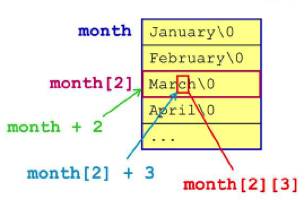
\includegraphics[width=5cm]{C/Untitled}}\tabularnewline
- grundlegende Datentypen (Tabelle oben) & - grundlegende Datentypen (Tabelle oben) & \tabularnewline
- Strukturen (struct) & - Strukturen (struct) & \tabularnewline
- Arrays & - Pointer & \tabularnewline
\cline{2-2} 
\multicolumn{1}{l|}{- Pointer} & \multicolumn{1}{l|}{ACHTUNG: Arrays können nicht zurückgegeben} & \tabularnewline
\multicolumn{1}{l|}{} & \multicolumn{1}{l|}{werden, jedoch Pointer auf Datenbereiche mit} & \tabularnewline
\multicolumn{1}{l|}{} & \multicolumn{1}{l|}{Arrays (char{*}, char{*}{*})} & \tabularnewline
\cline{2-2} 
\end{tabular}


\subsection*{Pointer}

\begin{tabular}{|l|ll|}
\hline 
int {*}p &  & Pointer auf int Objekt\tabularnewline
\hline 
double {*}d{[}20{]} &  & d= Array von 20 Pointer auf double-Objekte\tabularnewline
\hline 
double ({*}d){[}20{]} &  & d= Pointer auf ein double-Array mit 20 Objekten\tabularnewline
\hline 
char {*}{*}ppc &  & Pointer auf einen Pointer vom Typ char\tabularnewline
\hline 
double {*}cdp &  & Pointer auf double, {*}cdp=5.0, cdp++ möglich\tabularnewline
\hline 
double {*}const cdp &  & Konstanter Pointer, {*}cdp=5.0 möglich\tabularnewline
\hline 
const double {*}cdp &  & Pointer auf Konstante, {*}cdp++ möglich\tabularnewline
\hline 
const double {*}const cdp &  & Konstanter Pointer auf Konstante, keine Aktion\tabularnewline
\hline 
\end{tabular}
